
\documentclass[10pt]{report}
\usepackage{geometry} % see geometry.pdf on how to lay out the page. There's lots.
%\usepackage{natbib}
\usepackage{hyperref}
\usepackage{graphicx}
\newcommand{\tab}{\hspace*{2em}}
\geometry{a4paper} % or letter or a5paper or ... etc
\setlength\parindent{0pt}
% \geometry{landscape} % rotated page geometry

% See the ``Article customise'' template for come common customisations

\title{DupliPHY - User Guide}
\author{R. M. Ames}
\date{}

%%% BEGIN DOCUMENT
\begin{document}

\maketitle
\tableofcontents

\section{Change log}

{\bf Version 2.0.} Major update to the newick tree parser to accept a wider variety of newick formatted trees. Added extra exception handling to prevent uninformative program exits. Added a default gain and loss weights matrix which will be used if no matrix file is specified on the command line.
\\
\\
{\bf Version 1.0} Initial release.  

\section{License}

DupliPHY is licensed under GPL v3 (see gel.txt for more information).

\section{Citation}

If you use DupliPHY please cite \cite{ames2012determining}.

\section{Overview}

Recent large-scale studies of individuals within a population have demonstrated that there is wide-spread variation in copy number in many gene families.  In addition, there is increasing evidence that the variation in gene copy number can give rise to substantial phenotypic effects.  In some cases these variations have been shown to be adaptive.  These observations show that a full understanding of the evolution of biological function requires an understanding of gene gain and gene loss.  Accurate, robust evolutionary models of gain and loss events are, therefore, required.

We have developed weighted parsimony and maximum likelihood methods for inferring gain and loss events\cite{ames2012determining}. These methods have been tested on a range of simulated data and {\it Drosophila} data.  We have shown that maximum likelihood and weighted parsimony have similar accuracy for reconstructing the ancestral state.  For ancestral reconstruction we recommend weighted parsimony because it has similar accuracy to maximum likelihood, but is much faster.

\section{Installation}

DupliPHY has been implemented in Java 1.6 and is distributed as an executable jar file. As such there is no need for any complex installation, if java (version $>=$ 1.6) is installed the program should run on any platform. 

To check java is installed on your system type {\it java -version} at the command prompt. If an error message is displayed you can download and install java (version $>=$ 1.6) from the Oracle website (\url{http://www.oracle.com/us/technologies/java/overview/index.html}). 

Once java is installed simply download the DupliPHY jar file and follow the commands outlined in section \ref{sec:running}.

\section{Methods}

DupliPHY implements Sankoff's dynamic programming procedure \cite{sankoff1975locating}, to assign duplication and loss events on a phylogenetic tree. This algorithm uses a post-order tree-traversal and to assign each internal node a cost for each potential character at that node given the characters at the descendants of the node, followed by a pre-order tree-traversal to assign ancestral states.When calculating weighted parsimony with DupliPHY it is possible that multiple gene family sizes have the same parsimony score at the root. In cases of multiple family sizes having the same parsimony score at the root we arbitrarily choose the family with the fewest members. To ensure this choice does not affect the accuracy of DuliPHY we compared the accuracy of choosing the family with the fewest members to choosing a random family; we find there is little difference \cite{ames2012determining}. The program can use either a user defined matrix or a default matrix (as used in \cite{ames2012determining}) for the weights of gain and loss events.

\section{Input data}

DupliPHY has 3 mandatory inputs and one optional input.

\subsection{Family file}
\label{sec:family}

The family file is a tab delimited file containing a header line and then a line per family. The header line lists the species in the analysis. Each subsequent line indicates the number of members of that family present in each species. The first column of the file is reserved for a family ID. {\bf NB. All species listed in the family file must be present in the phylogenetic tree.}

\begin{quote}

FAMILY\tab dana\tab dere\tab dgri\tab dmel\tab dmoj\tab dpse\tab dsim\tab dvir\tab dyak\\
Fam1\tab\tab 1\tab\tab	1\tab\hspace{1em} 2\tab\tab	2\tab\tab	1\tab\hspace{1em}	1\tab\hspace{1em} 1\tab\hspace{1em}	1\tab\tab	2\\
Fam2\tab\tab 8\tab\tab	7\tab\hspace{1em} 6\tab\tab	5\tab\tab	6\tab\hspace{1em}	7\tab\hspace{1em} 2\tab\hspace{1em}	7\tab\tab	8\\

\end{quote}

\subsection{Tree file}
\label{sec:tree}

DupliPHY needs a phylogeny in order to infer the ancestral gene family sizes (Figure \ref{fig:tree}).

\begin{figure}
\centering
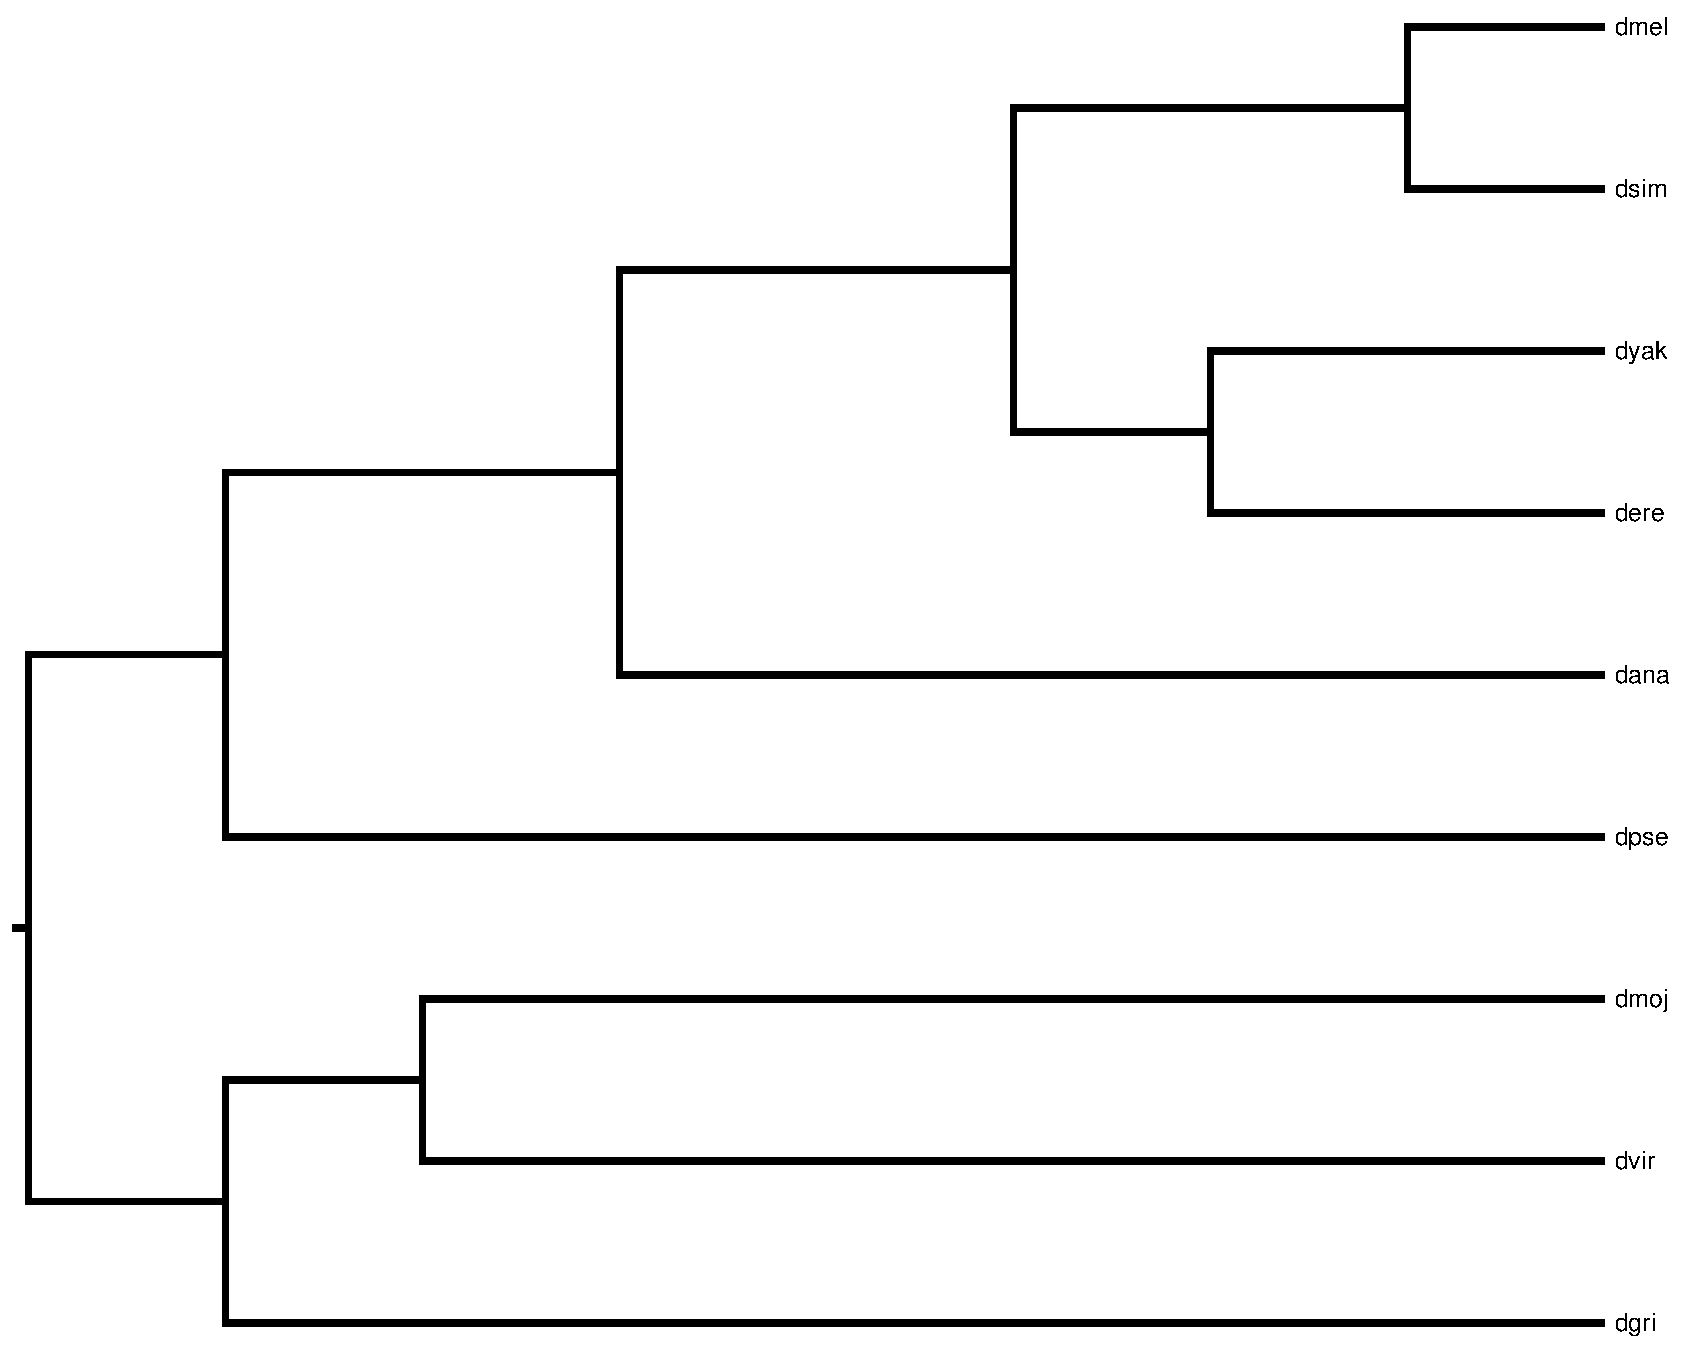
\includegraphics[width=0.75\textwidth]{tree.pdf}
\caption{Phylogenetic tree of 9 {\it Drosophila} species.}
\label{fig:tree}
\end{figure}

DupliPHY accepts newick formatted trees. The trees can either have labels on the internal nodes or these labels can be omitted. If no internal nodes labels are present DupliPHY will add these automatically and they will be included in the output. Any of the following trees will be accepted by DupliPHY. {\bf NB. All species in the phylogenetic tree must be present in the gene family file.}\\
\\
((((( dmel:1.0, dsim:1.0) A:2.0,( dyak:2.0, dere:2.0) B:1.0) C:2.0, dana:5.0) E:2.0, dpse:7.0) F:1.0,(( dmoj:6.0, dvir:6.0) G:1.0, dgri:7.0) H:1.0) Root:0.0; \\
\\
((((( dmel,dsim),(dyak,dere)),dana),dpse),((dmoj,dvir) dgri));\\
\\
(((((dmel:1.0, dsim:1.0) :1.0,(dyak:1.0, dere:1.0) :1.0) :1.0, dana:1.0) :1.0, dpse:1.0) :1.0,((dmoj:1.0, dvir:1.0) :1.0, dgri:1.0) :1.0);\\
\\

\subsection{Results prefix}
\label{sec:results}

The final mandatory option that the user must supply is a results prefix. This is simply the name that should be given to the results files.

\subsection{Matrix file (optional)}
\label{sec:matrix}

By providing a matrix file on the command line DupliPHY will use the user supplied weights to infer gain and loss events. The weights matrix must be a square matrix in the form:

\begin{quote}
0 \tab 1 \tab 2 \tab 3 \tab 4\\
1 \tab 0 \tab 1 \tab 2 \tab 3\\
2 \tab 1 \tab 0 \tab 1 \tab 2\\
3 \tab 2 \tab 1 \tab 0 \tab 1\\
4 \tab 3 \tab 2 \tab 1 \tab 0\\
\end{quote}

For rows ({\it i}) and columns ({\it j}) the matrix value at {\it i, j} defines the cost of a family changing from {\it i} members to {\it j} members. {\bf NB. The supplied matrix must be at least as large as the largest family in the family file as DupliPHY will not automatically expand a supplied matrix. For example if the largest family size is the dataset is 20 the matrix must be 20x20.}

If the matrix file is omitted from the command line DupliPHY will use the default weights matrix that can be generated from the input family file. This matrix was used in \cite{ames2012determining} and follows the same pattern as the matrix described above but extended to fit the gene family data.

\section{Running DupliPHY}
\label{sec:running}

DupliPHY is a command line tool where usage follows:

\begin{quote}
java -jar $<$family file$>$ $<$tree file$>$ $<$results prefix$>$ $<$matrix file$>$
\end{quote}

\begin{description}
	\item[family file] The tab delimited gene family file (see \ref{sec:family}). e.g. family.txt
	\item[tree file] The phylogenetic tree in newick format (see \ref{sec:tree}). e.g. tree.ph
	\item[results prefix] The prefix for the generated results files (see \ref{sec:results}). e.g. myResults
	\item[matrix file - optional] The matrix file with user defined weights for gains and losses (see \ref{sec:matrix}) e.g. matrix
\end{description}

To run DupliPHY on the supplied example data use:

\begin{quote}
java -jar family.txt tree.ph myResults matrix\\
OR\\
java -jar family.txt tree.ph myResults\\
\end{quote}

This will generate the results files with the prefix myResults.

\section{Outputs}

Running DupliPHY with the command listed in \ref{sec:running} will generate two output files:

\begin{description}
	\item[myResults\_desc.txt] A tab delimited gene family file showing the extant gene family sizes (as provided by the user) and the ancestral reconstruction at the internal nodes of the tree.
	\item[myResults\_tree.ph] A phylogenetic tree for each input gene family in newick format with the ancestral gene family sizes in the internal node labels. The tree can be viewed in a tree viewer such as fig tree (\url{http://tree.bio.ed.ac.uk/software/figtree/}) and the internal node values can be displayed to show the evolutionary history of a gene family (Figure \ref{fig:results_tree}).
\end{description}

\begin{figure}
\centering
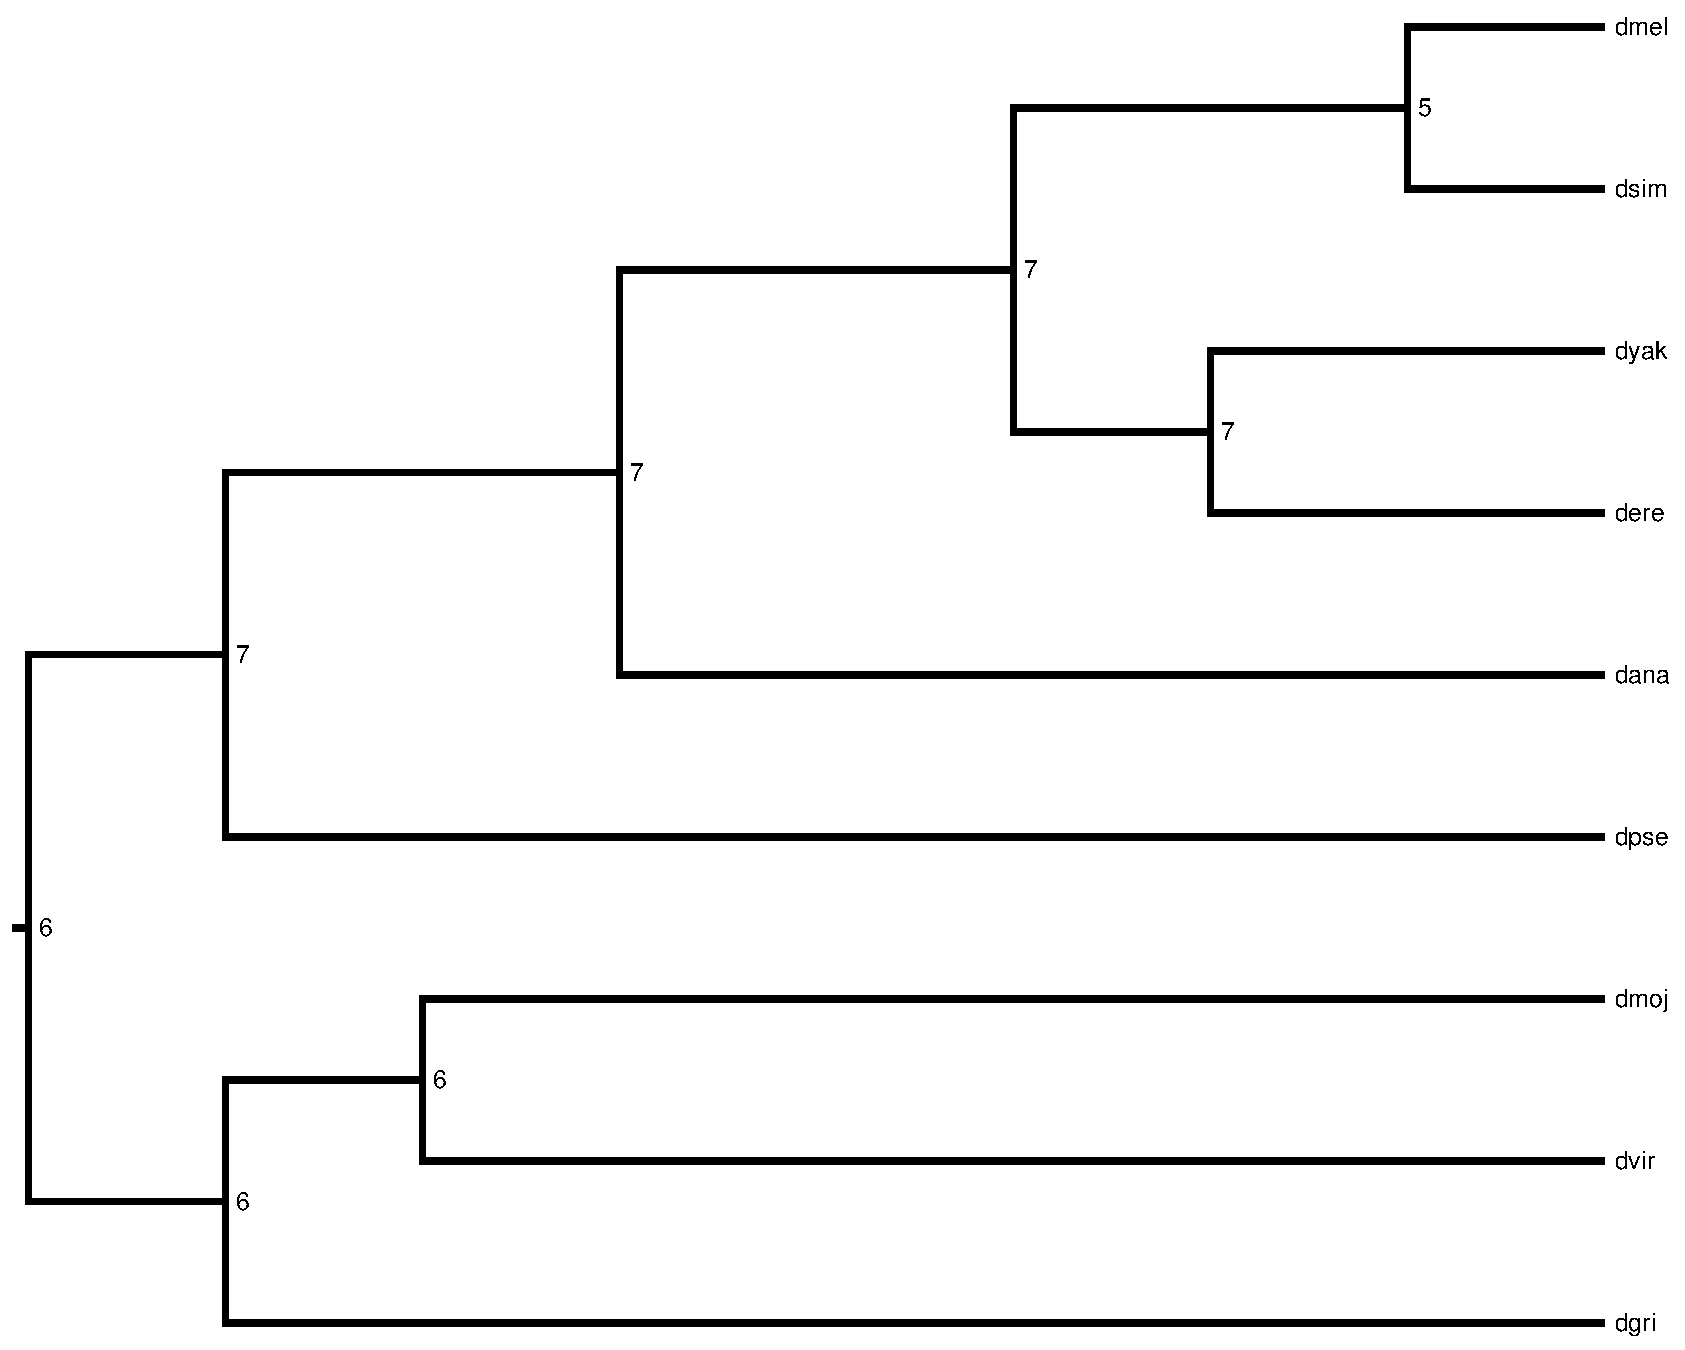
\includegraphics[width=0.75\textwidth]{results_tree.pdf}
\caption{Phylogenetic tree of 9 {\it Drosophila} species showing the ancestral reconstruction of Fam2.}
\label{fig:results_tree}
\end{figure}

\bibliographystyle{ieeetr}
\bibliography{bibliography}

\end{document}